\documentclass{zkdl-tests-template}

\title{\huge\sffamily\bfseries ZKDL Camp Exercises}
\author{\Large\sffamily Distributed Lab}
\date{\sffamily \today}
\titlepic{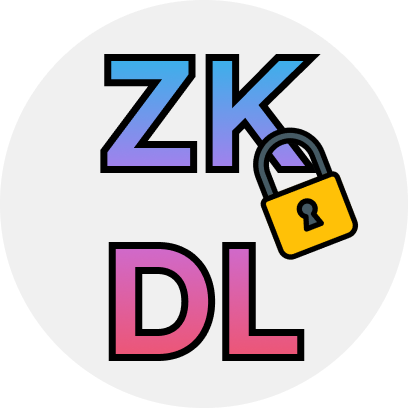
\includegraphics[width=0.2\textwidth]{../lectures/images/common/logo.png}}

\begin{document}

\pagestyle{fancy}

\maketitle

\pagebreak

\tableofcontents

\pagebreak

\section{Group Theory and Polynomials}

\subfile{1-math}

\section{Basics of Security Analysis}\label{section:math-crypto-2}

\subfile{2-math-and-crypto}

\section{Field Extensions and Elliptic Curves}

\subfile{3-ec}

\section{Projective Coordinates and Pairing}

\subfile{4-pairing}

\section{Commitment Schemes}

\subfile{5-commitments}

\section{Introduction to Zero-Knowledge Proofs}

\subfile{6-intro-zk}

\section{Sigma Protocols}

\subfile{7-sigma}

\section{Introduction to SNARKs. Arithmetic Circuits. R1CS}

\subfile{8-circuits}

\end{document}
